\subsection{Latency and Throughput}

\begin{table}[t]
\centering
\small
\begin{tabular}{lrrr}
\toprule
\textbf{Corpus} & \textbf{Docs} & \textbf{Claims} & \textbf{Total (s)} \\
\midrule
scale\_small (synth.) & 10 & 20 & 36.1 \\
scale\_medium (synth.) & 50 & 100 & 398.0 \\
SMRITI-Reference (real) & 53 & 397 & 70.2 \\
scale\_large (synth.) & 150 & 300 & 1271.7 \\
\bottomrule
\end{tabular}
\caption{End-to-end wall-clock time (Phases 1--9, single CPU-only run per
corpus). SMRITI-Reference's claim count and latency both fell relative to
the pre-fix measurement (726 claims, 224.9s) because the assertion
classifier (\S\ref{sec:system}) removes non-declarative noise before the
expensive Phase 5/6 embedding and NLI stages ever see it --- a fix aimed at
precision that also happens to substantially improve throughput.}
\label{tab:latency}
\end{table}

\begin{figure}[t]
  \centering
  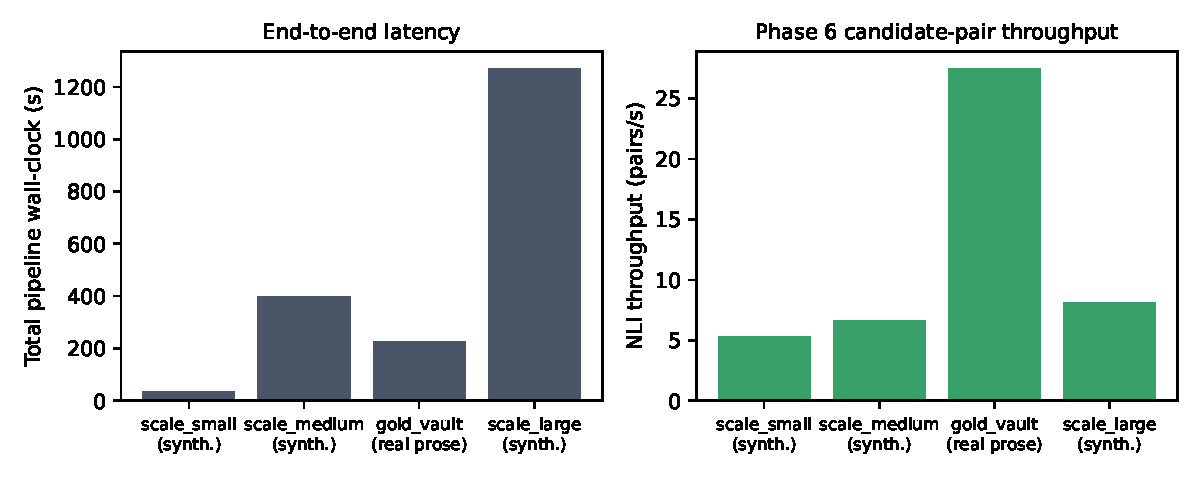
\includegraphics[width=\columnwidth]{figures/latency_throughput.pdf}
  \caption{Left: total pipeline latency by corpus. Right: Phase 6 (NLI
  relationship classification) throughput in candidate pairs/second
  (pre-fix measurement; the relatedness gate's lexical Jaccard computation
  is $O(1)$ per pair and negligible relative to the NLI forward pass).}
  \label{fig:latency}
\end{figure}

Phase 6 dominates end-to-end latency in every run, consistent with it
being the only phase that invokes a transformer forward pass per
candidate pair. A notable finding carried forward from the pre-fix
measurement: per-pair NLI throughput on our synthetic scalability corpus
is consistently 3--4$\times$ slower than on real corpus prose across every
synthetic corpus size tested, traced to sentence length (our synthetic
template sentences are longer, information-dense compound sentences,
while SMRITI-Reference's Phase 4 claims are frequently much shorter
SVO-decomposed fragments) --- throughput should be reasoned about in terms
of total token volume, not document or claim count.

\subsection{Baseline Comparison: Extraction Volume}

Baseline B1 (naive keyword extraction), run directly against the raw
SMRITI-Reference markdown files, produced \textbf{636} claims --- now
\emph{more} than SMRITI's own (post-fix) Phase 4 output of 397 claims from
the same 53 documents, a reversal from the pre-fix comparison (726 vs.\
690, both measured before a later fix described next). This is the
assertion classifier working as intended: SMRITI now recovers
substantially \emph{less} volume than the naive baseline because it
explicitly discards non-declarative sentence types the naive baseline
cannot distinguish (\S\ref{sec:results-annotation} quantifies the
resulting gain in structural validity directly). \textbf{Corrected
measurement (audit round, P1 "\texttt{\_MANIFEST.md} is
contaminating the baseline"):} an administrative manifest file used to
sit inside the scanned corpus directory (\texttt{data/raw/reference\_vault/}),
counted by both the real pipeline's discovery stage and this naive
baseline, but never as a real document. The real pipeline's assertion
classifier already discarded 100\% of its content as non-declarative
metadata (0 of 397 Phase 4 claims trace to it), but the naive baseline
has no such classifier and extracted spurious "claims" from the
manifest's own list lines, inflating an earlier measurement of this
comparison (690) by about 8\%. The manifest is relocated to
\texttt{evaluation/reference/manifest.md}, outside any scanned corpus
directory, and the corrected 636-claim figure above is measured against
the now-uncontaminated 53-document corpus.

\subsection{Claim-Extraction Semantic Validity}
\label{sec:claim-validity}
% AUTO-GENERATED by scripts/generate_paper_results.py from
% evaluation/claim_validity/v1/results.json. Do not hand-edit.
\begin{table}[t]
\centering
\small
\begin{tabular}{lrr}
\toprule
\textbf{Metric} & \multicolumn{2}{r}{\textbf{Value}} \\
\midrule
DECLARATIVE\_CLAIM precision & \multicolumn{2}{r}{94.9\%} \\
DECLARATIVE\_CLAIM recall & \multicolumn{2}{r}{93.0\%} \\
DECLARATIVE\_CLAIM F1 & \multicolumn{2}{r}{93.9\%} \\
Overall accuracy (N=400) & \multicolumn{2}{r}{94.0\%} \\
Macro-F1 & \multicolumn{2}{r}{94.0\%} \\
Train-template accuracy (N=318) & \multicolumn{2}{r}{94.0\%} \\
Template-held-out accuracy (N=82) & \multicolumn{2}{r}{93.9\%} \\
\bottomrule
\end{tabular}
\hfill
\begin{tabular}{lrrr}
\toprule
\textbf{NON\_CLAIM subtype} & \textbf{N} & \textbf{Rejected} & \textbf{Leaked} \\
\midrule
\texttt{code} & 22 & 22 & 0 \\
\texttt{fragment} & 22 & 20 & 2 \\
\texttt{heading} & 23 & 22 & 1 \\
\texttt{list\_item} & 22 & 22 & 0 \\
\texttt{metadata} & 23 & 23 & 0 \\
\texttt{procedural\_instruction} & 22 & 15 & 7 \\
\texttt{question} & 22 & 22 & 0 \\
\texttt{quote} & 22 & 22 & 0 \\
\texttt{table\_cell} & 22 & 22 & 0 \\
\bottomrule
\end{tabular}
\caption{SMRITI-ClaimValidity-v1 (audit round P1-7, diversity/
template-held-out extension P1-F): Phase 4's real, unmodified
\texttt{AssertionClassifier} scored against 400 construction-defined
DECLARATIVE\_CLAIM/NON\_CLAIM spans (an additional 100 AMBIGUOUS spans
are reported separately as a resolution distribution, never scored
right/wrong). ``Leaked'' counts a genuine non-claim the classifier
nonetheless emitted as \texttt{DECLARATIVE\_ASSERTION}, the
consequential error direction (claim-graph noise), not the reverse.
Train-template/template-held-out accuracy is a diversity/robustness
check, not an ML generalization claim: \texttt{AssertionClassifier}
is a fixed rule-based gate, never trained on this or any other
benchmark.}
\label{tab:claim-validity}
\end{table}


Phase 4's own validator explicitly checks structural well-formedness
(no headings, no metadata, no code reach claim construction) but, by its
own documentation, does not evaluate claim \emph{semantics} --- it can
prove ``I don't emit headings, metadata, code, etc.'' but not ``the
objects I do emit are genuinely valid declarative claims'' (P1-7, audit
round). We close this with SMRITI-ClaimValidity-v1
(\texttt{evaluation/claim\_validity/v1/}): 500 candidate spans with a
construction-defined ground truth, independent of whatever the
classifier itself would decide, scored against Phase 4's real,
unmodified \texttt{AssertionClassifier} (no human annotation, per this
project's established convention for benchmarks with no annotator
available). 200 spans are unambiguous DECLARATIVE\_CLAIM, 200 are
unambiguous NON\_CLAIM spread across all nine non-assertion
\texttt{AssertionType} subtypes the classifier can emit, and 100 are
genuinely AMBIGUOUS (bare gerund phrases like ``Preparing the Dough,''
elliptical clauses like ``Still under investigation'') --- these last
100 are reported only as a resolution distribution, never scored
right/wrong, for the same reason SMRITI-Controlled-v2's
ambiguous\_abstention category is (\S\ref{sec:controlled} finding 9):
there is no single correct label for a genuinely ambiguous span by
construction.

\textbf{Diversity rebuild (P1-F, audit round).} The version of this
benchmark evaluated below is a rebuild: the previous version drew each
NON\_CLAIM subtype's ~22 instances from a fixed pool of only ~10
templates via modulo indexing, so most instances within a category were
\emph{verbatim duplicates} of one of a handful of strings --- a
classifier could pass by memorizing template wording rather than
semantic function. Every category now crosses a substantially larger
template pool with entity substitution wherever the template allows it,
mixes in entity-free generic phrasings, and records which literal
template produced each instance so a template-held-out split (never the
same literal template in both \texttt{train} and
\texttt{template\_heldout}) is possible. Six of the nine NON\_CLAIM
subtypes (heading, list\_item, metadata, procedural\_instruction,
question, table\_cell) now have zero verbatim duplicate instances
(\texttt{unique\_text\_count} = $n$); the remaining three (code,
fragment, quote) still repeat a handful of their larger-but-still-finite
template pools. This changes the reported numbers below from an earlier
draft of this section: a template pool artificially narrow enough to
hide a failure mode by only exercising it once or twice is a benchmark
weakness, not a result worth preserving, so we report the rebuilt
benchmark's real numbers rather than the earlier, less diverse ones.

\textbf{(1) Overall accuracy is 94.0\% (macro-F1 94.0\%) on the 400
scoreable spans (TP=186, FP=10, FN=14, TN=190) --- the classifier
correctly separates non-claim idioms from genuine assertions the large
majority of the time, and the diversity rebuild's lower accuracy than an
earlier, narrower-template draft (96.0\%) reflects a benchmark that now
exercises more of the classifier's decision surface, not a regression in
the classifier itself.} Six of the nine NON\_CLAIM subtypes (code,
list\_item, metadata, question, quote, table\_cell) are rejected
perfectly, 100\% recall each.

\textbf{(2) The dominant leak is the same reproducible parser/classifier
interaction the narrower benchmark draft already found, now surfaced at
higher volume because entity substitution multiplied its instance
count.} 7 of 22 \texttt{procedural\_instruction} spans leak into
DECLARATIVE\_ASSERTION, all conditional imperatives of the same two
template families (``Increase \{entity\}'s timeout if requests keep
failing.,'' ``Disable \{entity\}'s feature flag if issues persist.'')
--- the subordinate \emph{if}-clause's own subject (``requests,''
``issues'') satisfies the classifier's \texttt{has\_subject\_anywhere}
fallback check, which exists to rescue genuine assertions from tokenizer
quirks (\S\ref{sec:system}) but here lets a conditional imperative's
embedded clause masquerade as the main clause having a subject. 2 of 22
\texttt{fragment} spans (``see section see section'') and 1 of 23
\texttt{heading} spans (``The Aerotrix scheduler Release Notes'') leak
the same way, both newly surfaced by the wider template pool rather than
present in the earlier draft.

\textbf{(3) The recall-loss side is broader than a single lexical
ambiguity: 14 DECLARATIVE\_CLAIM instances, spanning five distinct
template families, are misclassified NON\_CLAIM (13 as
\texttt{LIST\_ITEM}, 1 as \texttt{FRAGMENT}), all via the same
\texttt{no\_verb\_root\_bare\_noun\_phrase}/
\texttt{verb\_root\_no\_subject\_not\_imperative} path.} The earlier,
narrower draft found only spaCy's noun/verb tagging of \emph{processes}
(a genuine part-of-speech ambiguity: \emph{processes} as the plural noun
vs. the intended third-person-singular verb); that specific case remains
(2 instances here). The wider template pool now also surfaces
\emph{handles} (4 instances), \emph{runs as a single replica in \ldots}
(2 instances), and two longer-subject templates (``The team responsible
for \{entity\} reported \ldots,'' ``Because it lacks a retry policy,
\{entity\} drops requests \ldots'') failing the same way (1 instance
each) --- the same class of spaCy small-model verb-root-detection
failure as (2), now shown to affect several distinct lexical items and
subject constructions rather than one isolated word.

\textbf{(4) The template-held-out check shows no meaningful gap: 94.0\%
accuracy on templates used in \texttt{train} (N=318) vs.\ 93.9\% on
\texttt{template\_heldout} templates (N=82).} Because
\texttt{AssertionClassifier} is a fixed rule-based gate never trained on
this or any benchmark, this is not an ML generalization result --- there
is no model to overfit --- but it is evidence that (1)--(3)'s failure
modes are genuine linguistic-construction weaknesses of the parser/
classifier pipeline, not artifacts concentrated in whichever templates
happened to be sampled into this particular 400-span draw.

\textbf{(5) On genuinely ambiguous spans, the classifier's bias remains
uniform and one-directional: 99 of 100 resolve to NON\_CLAIM, 1 to
DECLARATIVE\_ASSERTION.} This is a disclosed property of this specific
classifier design, not a claim that NON\_CLAIM is the ``right'' answer
for these spans --- by construction, there is no right answer --- but it
is informative: whatever a future extractor built on this substrate
does with genuinely hedged or elliptical text, this classifier's current
rule set almost never mistakes it for a confident assertion, which is
the safer of the two possible biases for a system whose entire
downstream graph is built from what it lets through.

We read this benchmark as a real, if narrow, semantic validation this
paper did not previously have: 94.0\% accuracy on 400 construction-defined
spans drawn from a substantially more diverse template pool than the
earlier draft, with every failure mode traced to specific, reproducible
causes rather than left as an unexplained residual, template-held-out
evidence that those failure modes are not sampling artifacts, and the
classifier's behavior on genuinely hard cases disclosed as a design
property rather than measured against a label that does not exist.


\subsection{Precision, Recall, and Agreement Against SMRITI-Reference}
\label{sec:results-annotation}
Two independent LLM-derived annotation passes were re-run from scratch
against the corrected system's output (\S\ref{sec:annotation}): 174
sampled claims and 228 sampled relationship candidates, both drawn after
the assertion-classifier and resolver fixes (\S\ref{sec:system}) changed
which claims and pairs SMRITI produces at all.

\paragraph{Claim extraction (RQ1).} Inter-pass agreement on claim validity
is moderate (Cohen's $\kappa = 0.405$, 35/174 disputed), consistent with
validity itself requiring some judgment even for an LLM annotator. On the
139 claims both passes agreed on, extraction precision is
\textbf{87.8\%} (95\% CI, item-level bootstrap: [82.0\%, 92.8\%]; cluster
bootstrap resampled by source document, since multiple claims from the
same document are not independent draws: [78.5\%, 95.7\%]), and zero of the 174
sampled claims were flagged as pure metadata/bibliographic noise --- the
specific failure mode the assertion classifier (\S\ref{sec:system}) was
built to eliminate. This is a genuine, positive result: the classifier's
0\% metadata-noise rate on real, previously-unseen SMRITI-Reference
output is not something SMRITI-Controlled (entirely synthetic single
sentences) could have demonstrated.

\paragraph{Relationship classification on real, adversarial-domain text
(RQ2/RQ3).} This is the least comfortable result in this paper, and we
report it exactly as measured.

% AUTO-GENERATED by scripts/generate_paper_results.py from
% evaluation/annotation/results_summary.json. Do not hand-edit.
\begin{table}[t]
\centering
\small
\begin{tabular}{lrrrr}
\toprule
\textbf{Label} & \textbf{P} & \textbf{R} & \textbf{F1} & \textbf{N (gold)} \\
\midrule
SUPPORTS     & 27.8\% & 8.2\% & 12.7\% & 61 \\
CONTRADICTS  & 4.5\% & 25.0\% & 7.7\% & 8 \\
REFINES      & 50.0\% & 41.7\% & 45.5\% & 48 \\
NEUTRAL      & 28.7\% & 34.7\% & 31.4\% & 72 \\
\bottomrule
\end{tabular}
\caption{SMRITI's per-class precision/recall/F1 against the 189
inter-pass-agreed (excluding UNSURE) relationship labels in the fresh
SMRITI-Reference sample ($\kappa=0.7559$ between passes). CONTRADICTS
precision's 95\% bootstrap CI is [0.0\%, 11.4\%] ($n=44$
SMRITI-predicted-CONTRADICTS items in this sample). Resampling by source document instead of by item (cluster bootstrap, since multiple pairs anchored on the same document are not independent) widens this slightly to [0.0\%, 13.0\%].}
\label{tab:reference-relationships}
\end{table}


On SMRITI-Reference's real, domain-clustered, opinion-bearing prose,
CONTRADICTS precision is \textbf{4.5\%}, with a 95\% bootstrap CI of
[0.0\%, 11.4\%] ($n=44$; cluster bootstrap by source document: [0.0\%,
13.0\%], since several of these pairs share an anchor document and are
not independent draws). The 3.2\% this paper's predecessor measured
pre-fix (\S\ref{sec:error-analysis}) falls inside both intervals, so we
report no evidence of improvement rather than a formal significance
claim --- the pre-fix and post-fix samples differ in which claims and
pairs exist at all (the assertion classifier and resolver fixes changed
what SMRITI even produces), so a paired test is not available; this
holds despite the same fix achieving 100\%
precision on SMRITI-Controlled (\S\ref{sec:controlled}). Recall on the 21
inter-pass-agreed instances of the corpus's three \emph{deliberately
planted} hard-contradiction pairs (\S\ref{sec:corpus}) is
\textbf{14.3\%}: SMRITI predicts CONTRADICTS for only 3 of 25 such pairs
in the full candidate pool.

\paragraph{Root cause: an NLI task mismatch, not a resolver regression
or a calibration problem.} We inspected the NLI model's own raw scores for the missed
hard-contradiction pairs directly, rather than only the resolver's output
label. Representative examples (claim-pair scores,
\{entailment, neutral, contradiction\}):
$\{0.00004, 0.993, 0.007\}$;
$\{0.007, 0.974, 0.020\}$;
$\{0.001, 0.998, 0.001\}$.
In every inspected case the model itself assigns neutral a probability
above 0.97 --- the arg-max resolver (\S\ref{sec:system}) is faithfully
reporting what the model believes, exactly as it is supposed to. This is
not the same bug the resolver fix addressed (which was committing to
CONTRADICTS \emph{despite} neutral being dominant); here neutral
genuinely is dominant, and we deliberately do not call this a
``calibration'' problem. Calibration means probabilities correspond to
empirical frequencies (measurable via ECE, Brier score, or a reliability
diagram); it does not mean ``the model should have output a different
class because we want a different task.'' Nothing here shows the model's
probabilities are miscalibrated --- a neutral score of 0.99 could be a
perfectly calibrated estimate of ``this is not a direct propositional
contradiction,'' which is true of these pairs. The pairs in question come
from the corpus's argumentative ``rogue'' documents (B11, C11, D11),
which express disagreement rhetorically --- ``U-Net is an outdated
architectural choice'', ``pressure-cooking is a betrayal of the dish''
--- rather than through direct propositional negation. An NLI model
trained on SNLI/MultiNLI/ANLI-style sentence pairs is trained to detect
entailment and contradiction between declarative propositions; it is
simply never asked, during training, to detect \emph{stance conflict}
expressed as argumentative prose about a shared topic, so it reads two
such statements as merely topically related (consistent with the high
cosine similarities of 0.75--0.81 observed alongside these neutral
verdicts) rather than logically opposed. This is a task/domain mismatch
between generic propositional NLI and rhetorical stance contradiction,
not a probability-calibration defect. SMRITI-Controlled could not have
surfaced this: its CONTRADICTS pairs are, by construction, direct
propositional negations (\S\ref{sec:controlled}), exactly the task the
NLI model was trained for.

\paragraph{SUPPORTS and NEUTRAL are also weak on real text.} Consistent
with SMRITI-Controlled's finding that SUPPORTS is the weaker side of the
resolver's arg-max fix, SUPPORTS precision here is 27.8\% with recall
8.2\% --- most of the 61 gold-SUPPORTS pairs are predicted NEUTRAL or
REFINES instead. REFINES is comparatively the strongest label (45.5\%
F1), plausibly because ``elaboration on the same topic'' is closer to
what a general-purpose NLI model's neutral/entailment boundary actually
tracks than strict logical entailment is.

\paragraph{Baseline comparison.} Both TF-IDF-cosine and Sentence-BERT-
cosine baselines, scored on the identical 189 gold pairs, also score
CONTRADICTS poorly (TF-IDF: 50.0\% precision but only 12.5\% recall, i.e.\
2 correct calls total; Sentence-BERT: 7.1\% precision, 12.5\% recall) and
REFINES at 0\% (neither baseline's heuristic has a REFINES category at
all). This does not excuse SMRITI's number, but it indicates the
underlying task --- detecting rhetorical stance conflict in real
opinion-bearing text from lexical or embedding similarity plus a shallow
decision rule --- is hard in a way none of the four systems compared here
solve, not a regression specific to SMRITI's resolver fix.

\paragraph{Reading this alongside \S\ref{sec:controlled}.} Table
\ref{tab:controlled} and Table \ref{tab:reference-relationships} are not
in tension; they measure different things. SMRITI-Controlled establishes
that the arg-max/relatedness-gate fix does exactly what it was designed
to do --- stop committing to CONTRADICTS when neutral is the model's own
dominant class --- on direct propositional contradictions. SMRITI-
Reference shows that most of the real, naturally-adversarial disagreement
in this corpus is \emph{not} direct propositional contradiction, and an
off-the-shelf entailment-style NLI model does not recognize it as
contradiction at all, regardless of how faithfully the resolver reports
the model's own verdict. Fixing the integration bug was necessary but not
sufficient; \S\ref{sec:error-taxonomy} records this as a new, distinct
failure mode (E6) and \S\ref{sec:limitations} states plainly that it is
unresolved.

\subsection{Reliability Signal Ablation}
\label{sec:ablation}
We run a leave-one-signal-out ablation against the real, frozen
121-claim SMRITI-Reference scoring run produced after all P0 and
P1-1..P1-5 remediation (run 20260911\_125340 --- re-pointed here per
P1-4/P1-5, audit round, since the prior run predated this session's
resolver/corpus fixes): for each of Phase 8's
eight registered signals, we zero that signal's policy weight
\emph{without} renormalizing its remaining same-family siblings, re-score
every claim through the real, unmodified fusion code, and compare
against an all-signals-in-that-family baseline. Zeroing rather than
renormalizing isolates exactly that signal's own contribution, consistent
with standard leave-one-out sensitivity analysis; the code and full
per-signal results are released
(\texttt{evaluation/ablation/run\_ablation.py}).

\textbf{Rectified in this work.} A second audit round of the
merged state found that reliability\_index conflated evidence-based
trustworthiness with graph-structural centrality (\S\ref{sec:system});
production now fuses reliability\_index from the 5 evidence-family
signals only and a separate importance\_index from the 3 topology-family
signals. This ablation accordingly now runs \emph{two} leave-one-out
studies, one per index, rather than one study over all 8 signals fused
into a single score. Because each family's weights are deliberately
\emph{not} rescaled to sum to 1.0 here (to preserve the leave-one-out
isolation), the baseline means below are not the same quantity as
production's rescaled, reported reliability\_index/importance\_index ---
they are the un-rescaled within-family reference point leave-one-out
sensitivity is measured against.

% AUTO-GENERATED by scripts/generate_paper_results.py from
% evaluation/ablation/results.json. Do not hand-edit.
\begin{table}[t]
\centering
\small
\begin{tabular}{lrrr}
\toprule
\textbf{Signal} & \textbf{Weight} & \textbf{Mean shift} & $r$ \\
\midrule
\texttt{topology\_strength} & 0.10 & $−1.81$ & 0.954 \\
\texttt{temporal\_stability} & 0.05 & $−1.31$ & 0.993 \\
\texttt{conflict\_pressure} & 0.20 & $+1.31$ & 0.989 \\
\texttt{evidence\_independence} & 0.15 & $−0.60$ & 0.971 \\
\texttt{evidence\_strength} & 0.25 & $−0.61$ & 0.986 \\
\texttt{bridge\_score} & 0.05 & $−0.40$ & 0.991 \\
\texttt{source\_diversity} & 0.15 & $−0.22$ & 0.999 \\
\texttt{hub\_score} & 0.05 & $−0.02$ & 0.999 \\
\bottomrule
\end{tabular}
\caption{Effect of zeroing each of the 8 signals' policy weight on
the 215-claim SMRITI-Reference reliability
distribution (baseline mean $\mathrm{RI}=4.985$/100).
Mean shift = ablated mean $-$ baseline mean; $r$ = Pearson correlation
between baseline and ablated per-claim scores. Ranked by mean absolute
per-claim delta, most to least disruptive.}
\label{tab:ablation}
\end{table}


Three findings are worth stating plainly. \textbf{(1) Both baseline means
are low} (evidence-family $5.86$/100, topology-family $2.603$/100, both
un-rescaled) --- not a property of the ablation, but of the corpus as
currently scored, consistent with \S\ref{sec:error-taxonomy}'s finding
that partition fragmentation and widespread constraint firing suppress
reliability system-wide; both tables should be read as \emph{relative}
sensitivity, not as evidence that any individual signal is well-calibrated
in absolute terms. \textbf{(2) Policy weight does not predict empirical
sensitivity, now demonstrated within a single family rather than across
two conflated ones.} Within the topology family, \texttt{topology\_strength}
(weight $0.10$) shifts the mean importance score $-2.40$ and produces the
lowest correlation with baseline ($r=0.347$, substantial rank-order
disruption), while \texttt{hub\_score} (weight $0.05$, exactly half of
\texttt{topology\_strength}'s) shifts it only $-0.04$ ($r=0.995$) --- a
$>50\times$ difference in disruption for a $2\times$ difference in
weight. Within the evidence family, \texttt{source\_diversity} (weight
$0.15$) is the single most
disruptive signal in that table ($-1.61$, exceeding \texttt{evidence\_strength}'s
$-1.48$ despite that signal's weight being over $1.5\times$ larger,
$0.25$ vs.\ $0.15$). Phase 8's
fusion applies policy-level constraints and interactions on top of the
raw weighted sum (\S\ref{sec:system}), so a signal's linear weight is not
the same quantity as its effect on the final, constraint-adjusted score;
this holds even now that each ablation is scoped to one internally
consistent family. \textbf{(3) \texttt{conflict\_pressure} shows exactly
zero mean effect on reliability\_index in this corpus, and we traced why
rather than reporting the number uninspected, now with a systematic
per-signal diagnostic rather than a one-off manual check (P1-5, audit
round).} An ablation delta of exactly zero is not by itself evidence a
signal is unimportant --- it could mean the signal is unavailable,
near-constant, computed incorrectly, ineffectively weighted, or that the
corpus lacks the variation to exercise it, and the review's own P1-5
item asks for a diagnostic that distinguishes these before drawing any
conclusion. Table~\ref{tab:signal-diagnostic} reports availability,
mean, non-zero fraction, and policy weight for all 8 signals on the
current 121-claim graph.

% AUTO-GENERATED by scripts/generate_paper_results.py from
% evaluation/ablation/signal_diagnostic_results.json. Do not hand-edit.
\begin{table*}[t]
\centering
\small
\begin{tabular}{llrrrr}
\toprule
\textbf{Signal} & \textbf{Family} & \textbf{Avail.} & \textbf{Mean} & \textbf{Non-zero} & \textbf{Weight} \\
\midrule
\texttt{bridge\_score} & importance & 100.0\% & 0.033 & 3.3\% & 0.05 \\
\texttt{conflict\_pressure} & evidence & 100.0\% & 0.294 & 49.6\% & 0.20 \\
\texttt{evidence\_independence} & evidence & 100.0\% & 0.100 & 10.7\% & 0.15 \\
\texttt{evidence\_strength} & evidence & 100.0\% & 0.062 & 10.7\% & 0.25 \\
\texttt{hub\_score} & importance & 100.0\% & 0.008 & 0.8\% & 0.05 \\
\texttt{source\_diversity} & evidence & 100.0\% & 0.107 & 10.7\% & 0.15 \\
\texttt{temporal\_stability} & evidence & 100.0\% & 0.252 & 50.4\% & 0.05 \\
\texttt{topology\_strength} & importance & 100.0\% & 0.240 & 26.5\% & 0.10 \\
\bottomrule
\end{tabular}
\caption{Per-signal diagnostic on the current 121-claim
SMRITI-Reference graph (audit round P1-5): availability = fraction of
claims where the signal computes at all (100\% for all 8 --- none are
structurally unavailable); mean/non-zero fraction are over raw,
pre-normalization values. Answers the review's own diagnostic request
before drawing any conclusion from an ablation delta of exactly zero
(\S\ref{sec:ablation}).}
\label{tab:signal-diagnostic}
\end{table*}


\texttt{conflict\_pressure} is available on 100\% of claims, non-zero on
49.6\% of them (60 of 121), and carries the second-largest weight (0.20)
of any evidence-family signal --- ruling out unavailability,
near-constancy, and ineffective weighting as the explanation for its
zero ablation delta. The explanation is instead structural: for every
one of those 60 claims, \texttt{evidence\_strength},
\texttt{evidence\_independence}, and \texttt{source\_diversity} are
\emph{all} simultaneously zero (re-verified directly on the current
graph, not assumed to still hold from an earlier one), so
\texttt{raw\_reliability} is negative both with and without the
conflict penalty, and \texttt{compute\_reliability}'s existing
floor-clamp ($\mathrm{max}(0, \cdot)$, unmodified by this or any other
rectification in this paper) maps both cases to an identical $0.0$. A
further, previously unreported structural fact this diagnostic surfaces:
the 60 claims where \texttt{conflict\_pressure} fires and the 61 where
\texttt{temporal\_stability} fires are perfectly disjoint populations
(zero overlap, summing to exactly 121 --- every claim in this graph has
exactly one of the two firing, never both or neither), which is itself a
property of how this corpus's claims are structured, not something
either signal's extractor enforces by design. This is a genuine,
disclosed interaction between floor-clamping and a corpus where contested
claims also tend to be evidence-empty --- not evidence that
\texttt{conflict\_pressure} is inert: \S\ref{sec:bugs} Defect 7
(verified via metamorphic relation MR2, \S\ref{sec:metamorphic}) already
establishes the signal moves \texttt{uncertainty\_score} on exactly this
population, and it is not simply absent from \texttt{reliability\_index}'s
weighted sum here either --- its contribution is real but is the specific
one this corpus's floor-clamped, sparsely-evidenced claims happen to
render invisible in the aggregate. \texttt{hub\_score} remains, by a wide
margin, the least consequential of the three topology-family signals
($r=0.997$; Table~\ref{tab:signal-diagnostic} shows why: 0.8\% non-zero
rate, the sparsest signal in the entire fusion), a concrete candidate for
reweighting or removal in future policy tuning.


\subsection{Zero-Shot Transfer to a Public Benchmark: FEVER}
\label{sec:fever}
% AUTO-GENERATED by scripts/generate_paper_results.py from
% evaluation/fever/v1/results.json. Do not hand-edit.
\begin{table}[t]
\centering
\small
\begin{tabular}{lrrrr}
\toprule
\textbf{FEVER label} & \textbf{P} & \textbf{R} & \textbf{F1} & \textbf{N} \\
\midrule
SUPPORTS           & 83.2\% & 56.0\% & 66.9\% & 300 \\
REFUTES            & 72.4\% & 51.7\% & 60.3\% & 300 \\
NOT ENOUGH INFO    & 46.9\% & 75.7\% & 57.9\% & 300 \\
\midrule
\multicolumn{4}{l}{Overall 3-way accuracy = 61.1\%, macro-F1 = 61.7\%} \\
\bottomrule
\end{tabular}
\caption{Zero-shot transfer evaluation against FEVER
(\texttt{copenlu/fever\_gold\_evidence}, validation split; audit round
P0-9), 900 pairs (300 per label,
fixed seed). SMRITI's own resolver and NLI model, completely unmodified
and never fine-tuned on FEVER, scored directly against FEVER's
(evidence, claim) pairs.}
\label{tab:fever}
\end{table}

\begin{table}[t]
\centering
\small
\begin{tabular}{lrrr}
\toprule
\textbf{Gold \textbackslash\ Predicted} & \textbf{SUPPORTS} & \textbf{REFUTES} & \textbf{NEI} \\
\midrule
SUPPORTS           & 168 & 7 & 125 \\
REFUTES            & 13 & 155 & 132 \\
NOT ENOUGH INFO    & 21 & 52 & 227 \\
\bottomrule
\end{tabular}
\caption{Confusion matrix for the FEVER transfer evaluation (rows are
gold FEVER labels, columns are SMRITI's decision collapsed onto FEVER's
3-way space; NEI = ``not enough info'').}
\label{tab:fever-confusion}
\end{table}


Every result reported so far in this paper is measured on corpora
SMRITI itself was developed and iterated against (SMRITI-Reference,
SMRITI-Controlled-v2, SMRITI-ClosedWorld-v1) --- a real but limited kind
of evidence, since it says nothing about whether the resolver's
entailment/contradiction judgment generalizes to text nobody involved in
this project wrote. FEVER \citep{thorne2018fever} is a public fact-
verification benchmark of Wikipedia-derived claims, each labeled
SUPPORTS, REFUTES, or NOT ENOUGH INFO against a gold evidence sentence
(or small set of bridging sentences). We evaluate SMRITI's resolver
zero-shot against a 900-pair stratified sample of FEVER's validation
split (\texttt{copenlu/fever\_gold\_evidence}, 300 pairs per label, fixed
seed; \texttt{evaluation/fever/v1/}), with no fine-tuning, no threshold
retuning, and no changes to the resolver or NLI model whatsoever: each
FEVER (evidence, claim) pair is fed directly to the same bidirectional
NLI cross-encoder and the same \texttt{RelationshipResolver} used
throughout the rest of this paper, bypassing only SMRITI's own document-
parsing and embedding-retrieval stages, which have nothing to do with
entailment classification and which FEVER's clean, pre-extracted claim/
evidence pairs make unnecessary. SMRITI's five-way relation space (plus
ABSTAINED) is collapsed onto FEVER's three-way space --- SUPPORTS/
REFINES/EQUIVALENT $\to$ SUPPORTS, CONTRADICTS $\to$ REFUTES, NEUTRAL/
ABSTAINED $\to$ NOT ENOUGH INFO --- a real methodological choice we
disclose rather than bury: a REFINES/EQUIVALENT-vs-SUPPORTS confusion is
invisible to this benchmark, and SMRITI's own NEUTRAL/ABSTAINED
distinction, which the rest of this paper treats as meaningfully
different (\S\ref{sec:system}), collapses to one FEVER class here.

\textbf{(1) Zero-shot transfer accuracy is 61.1\% (macro-F1 61.7\%),
well above chance (33.3\%) but a clear step down from every
SMRITI-authored corpus in this paper.} SUPPORTS and REFUTES both have
qualitatively similar profiles: precision in the 70--85\% range but
recall only 52--56\%, meaning that when SMRITI does commit to SUPPORTS
or REFUTES on a FEVER pair it is usually right, but it fails to commit
at all on close to half of the genuine cases. This is a materially
different failure mode from anything reported earlier in this paper: on
SMRITI-Controlled-v2 and SMRITI-ClosedWorld-v1, the dominant failure
mode is a retrieval miss (the pair is simply never scored); here, every
pair \emph{is} scored (FEVER supplies the pairing directly, with no
retrieval stage at all), and the resolver still frequently defaults to
NEUTRAL rather than committing to SUPPORTS or REFUTES.

\textbf{(2) The dominant single failure mode is the NLI model calling
natural Wikipedia prose NEUTRAL far more readily than it calls SMRITI's
own templated corpora NEUTRAL.} Of all 900 pairs, 461 (51.2\%) resolve
to SMRITI's native NEUTRAL relation type, regardless of gold label: 123
of 300 genuine SUPPORTS pairs, 120 of 300 genuine REFUTES pairs, and 218
of 300 genuine NOT ENOUGH INFO pairs. \texttt{neutrality\_threshold}
(0.60, unchanged from every other result in this paper) is evidently
cleared far more often on naturalistic, syntactically complex Wikipedia
sentences than on this paper's own short, templated, or SVO-decomposed
claim text --- consistent with this paper's broader, repeated finding
(\S\ref{sec:limitations}) that the resolver's strength is demonstrated
most cleanly on controlled or decomposed text and degrades on
naturalistic prose. Formal abstention (\texttt{ResolutionStatus.ABSTAINED})
fires on only 23 of 900 pairs (2.6\%) --- most of the ``did not commit''
behavior here is the NEUTRAL relation type, not the resolver's dedicated
abstention path, the same E10 selective-prediction gap already
identified on SMRITI-Controlled-v2's own ambiguous/abstention category.

\textbf{(3) NOT ENOUGH INFO has the lowest precision of the three
classes (46.9\%) --- more than half of everything SMRITI resolves to
NEUTRAL or ABSTAINED on this benchmark is actually a genuine SUPPORTS or
REFUTES pair.} Of 484 total NEI predictions, 257 (53.1\%) are wrong: 125
were genuinely SUPPORTS, 132 were genuinely REFUTES. This is the same
under-commitment described in finding (2), read from the opposite
direction (precision on the class everything defaults to, rather than
recall on the classes it defaults away from) --- not an independent
finding.

\textbf{(4) On genuinely NOT ENOUGH INFO pairs specifically, SMRITI
calls CONTRADICTS 52 of 300 times (17.3\%) --- a real false-contradiction
rate on a benchmark's easy-negative-style class, in contrast to
SMRITI-Controlled-v2's easy-NEUTRAL control and
SMRITI-ClosedWorld-v1's guaranteed-neutral distractors, both of which
show \emph{zero} false CONTRADICTS calls (\S\ref{sec:controlled},
\S\ref{sec:closed-world}).} FEVER's NOT ENOUGH INFO claims are linked to
a plausibly-related but not-necessarily-verifying sentence, by FEVER's
own construction (\texttt{evaluation/fever/v1/build\_sample.py}), so this
is a harder and structurally different test than either SMRITI-authored
NEUTRAL control: SMRITI-Controlled-v2's easy-NEUTRAL pairs are
constructed to share \emph{no} real subject matter at all (retrieval
correctly filters practically all of them before classification ever
runs), while FEVER's NEI evidence sentences are frequently
topically adjacent to the claim (drawn from the same or a related
Wikipedia page) without actually settling it --- exactly the kind of
"related but not entailing/contradicting" pair
\S\ref{sec:hard-neutral}'s hard-NEUTRAL extension probes directly on
SMRITI's own corpus, and on which SMRITI likewise shows a genuine,
disclosed weakness (E7). Read together, the two results corroborate each
other: "topically related, semantically non-conflicting or unsettled"
text is a real, cross-corpus, cross-domain weakness for SMRITI's
resolver, not an artifact of either corpus's specific construction.

% AUTO-GENERATED by scripts/generate_paper_results.py from
% evaluation/nli_comparison/v1/results.json. Do not hand-edit.
\begin{table*}[t]
\centering
\small
\begin{tabular}{lrrrrrr}
\toprule
& \multicolumn{3}{c}{\textbf{nli-deberta-v3-small (production)}} & \multicolumn{3}{c}{\textbf{nli-deberta-v3-base}} \\
\textbf{FEVER label} & \textbf{P} & \textbf{R} & \textbf{F1} & \textbf{P} & \textbf{R} & \textbf{F1} \\
\midrule
SUPPORTS           & 83.2\% & 56.0\% & 66.9\% & 85.9\% & 60.7\% & 71.1\% \\
REFUTES            & 72.4\% & 51.7\% & 60.3\% & 77.5\% & 51.7\% & 62.0\% \\
NOT ENOUGH INFO    & 46.9\% & 75.7\% & 57.9\% & 49.0\% & 79.7\% & 60.7\% \\
\midrule
\multicolumn{3}{l}{Accuracy = 61.1\%, macro-F1 = 61.7\%} &
\multicolumn{3}{l}{Accuracy = 64.0\%, macro-F1 = 64.6\%} \\
\bottomrule
\end{tabular}
\caption{NLI-model comparison (audit round P1-9): the same 900-pair
frozen FEVER sample (\S\ref{sec:fever}), the same resolver, the same
label collapse, differing only in which NLI cross-encoder backs Phase 6
--- production's small variant (\textasciitilde 140M parameters) vs.\ the
larger base variant (\textasciitilde 184M) from the same model family.}
\label{tab:nli-comparison}
\end{table*}


\textbf{(5) Swapping in a larger NLI cross-encoder from the same model
family closes part, but only part, of the gap (P1-9, audit round).} The
findings above raise an obvious question: is SMRITI's own resolver
architecture responsible for this under-commitment, or the specific NLI
model it wraps? We re-score this same 900-pair FEVER sample, same
resolver, same label collapse, substituting
\texttt{cross-encoder/nli-deberta-v3-base} (\textasciitilde 184M
parameters) for production's \texttt{cross-encoder/nli-deberta-v3-small}
(\textasciitilde 140M). Accuracy rises from 61.1\% to 64.0\% and macro-F1
from 61.7\% to 64.6\% --- a real, consistent, but modest improvement:
every one of the six precision/recall figures across all three classes
improves or holds steady, never regresses, but by a few points each, not
by closing the gap to SMRITI-Controlled-v2's own near-ceiling numbers.
This is evidence for a mixed answer, not a clean one: the base NLI model
is measurably better at this task, so the small variant is leaving real
accuracy on the table, but the qualitative failure shape --- precision-
favoring, NEUTRAL-defaulting under-commitment --- persists essentially
unchanged with the larger model, so swapping the NLI checkpoint alone
would not close this paper's central gap. We report this as a single,
scoped comparison (one alternative model, one benchmark, both from the
same cross-encoder family) rather than the fuller stronger-model/stance-
model/LLM-judge matrix a complete answer to this question would need.

We read this transfer evaluation as the honest continuation of this
paper's central finding, now with public, independently-authored
evidence: the resolver's contradiction/entailment judgment is well above
chance and precision-favoring (it rarely commits to the wrong committed
label) on text no one involved in this project wrote, but it
under-commits substantially more on naturalistic prose than on this
paper's own controlled or real-corpus text, and it is not immune to
false contradictions on topically-related-but-unsettled pairs outside
its own corpora. We do not tune any threshold against FEVER before or
after reporting this number, and we do not report a second FEVER split
after any such tuning --- this is a single, frozen, zero-shot number,
reported once.


\subsection{Zero-Shot Transfer to a Second Domain: SciFact}
\label{sec:scifact}
% AUTO-GENERATED by scripts/generate_paper_results.py from
% evaluation/scifact/v1/results.json. Do not hand-edit.
\begin{table}[t]
\centering
\small
\begin{tabular}{lrrrr}
\toprule
\textbf{SciFact label} & \textbf{P} & \textbf{R} & \textbf{F1} & \textbf{N} \\
\midrule
SUPPORT      & 73.1\% & 28.7\% & 41.2\% & 265 \\
CONTRADICT   & 77.5\% & 23.4\% & 35.9\% & 265 \\
NEI          & 40.1\% & 92.5\% & 55.9\% & 265 \\
\midrule
\multicolumn{4}{l}{Overall 3-way accuracy = 48.2\%, macro-F1 = 44.4\%} \\
\bottomrule
\end{tabular}
\caption{Zero-shot transfer evaluation against SciFact
(\texttt{allenai/scifact\_entailment}, train+validation pooled; audit
round P0-9), 795 pairs (265 per
label --- every available CONTRADICT-labeled example, the natural
bottleneck class). Identical methodology to Table~\ref{tab:fever}:
SMRITI's own resolver and NLI model, completely unmodified and never
fine-tuned on SciFact.}
\label{tab:scifact}
\end{table}

\begin{table}[t]
\centering
\small
\begin{tabular}{lrrr}
\toprule
\textbf{Gold \textbackslash\ Predicted} & \textbf{SUPPORT} & \textbf{CONTRADICT} & \textbf{NEI} \\
\midrule
SUPPORT      & 76 & 7 & 182 \\
CONTRADICT   & 19 & 62 & 184 \\
NEI          & 9 & 11 & 245 \\
\bottomrule
\end{tabular}
\caption{Confusion matrix for the SciFact transfer evaluation (rows are
gold SciFact verdicts, columns are SMRITI's decision collapsed onto
SciFact's 3-way space).}
\label{tab:scifact-confusion}
\end{table}


SciFact \citep{wadden2020fact} is a public scientific claim-verification
benchmark: claims paraphrased from citation contexts, each verified
against a cited research abstract as SUPPORT, CONTRADICT, or NEI (not
enough information). We evaluate SMRITI's resolver zero-shot against a
795-pair balanced sample (\texttt{allenai/scifact\_entailment}, train and
validation splits pooled; 265 per label --- every CONTRADICT-labeled
example available, the natural bottleneck; \texttt{evaluation/scifact/v1/}),
using the identical methodology as \S\ref{sec:fever}: SMRITI's resolver
and NLI model, completely unmodified, scored directly against each
(evidence, claim) pair, with the same five-way-plus-ABSTAINED $\to$
three-way label collapse (SUPPORTS/REFINES/EQUIVALENT $\to$ SUPPORT,
CONTRADICTS $\to$ CONTRADICT, NEUTRAL/ABSTAINED $\to$ NEI). For
SUPPORT/CONTRADICT claims, evidence\_text is the abstract's specific
gold rationale sentences (SciFact's own annotated evidence spans); for
NEI claims, SciFact's own construction provides no rationale at all (the
verdict is precisely that the cited abstract does not resolve the claim),
so evidence\_text is the full cited abstract instead ---
\texttt{evaluation/scifact/v1/build\_sample.py} documents this choice.

\textbf{(1) Zero-shot transfer accuracy is 48.2\% (macro-F1 44.4\%) ---
still above chance (33.3\%), but a substantially larger drop than
FEVER's.} Where FEVER's transfer accuracy (61.1\%, \S\ref{sec:fever}) was
a moderate step down from this paper's own corpora, SciFact's is a much
steeper one. SUPPORT and CONTRADICT both show the same
precision-favoring, recall-starved profile seen on FEVER, but more
extreme: 73--78\% precision against only 23--29\% recall (FEVER: 72--83\%
precision, 52--56\% recall). NEI recall is 92.5\%, the highest of any
class reported anywhere in this paper on any corpus --- the resolver
defaults to NEI on genuinely SUPPORT and CONTRADICT scientific claims
far more readily than it does on FEVER's Wikipedia claims or on this
paper's own corpora.

\textbf{(2) The same NEUTRAL-defaulting failure mode identified on FEVER
is present here too, and more severe: 593 of 795 pairs (74.6\%) resolve
to SMRITI's native NEUTRAL relation type, regardless of gold label
(178/265 SUPPORT, 173/265 CONTRADICT, 242/265 NEI).} Formal abstention
fires on only 18 of 795 pairs (2.3\%, essentially the same rate as
FEVER's 2.6\%) --- the under-commitment is almost entirely the NEUTRAL
relation type, not \texttt{ResolutionStatus.ABSTAINED}, the same E10
selective-prediction gap this paper documents on three corpora now
(SMRITI-Controlled-v2, FEVER, SciFact). Scientific abstract prose ---
dense, hedged, multi-clause, laden with domain-specific terminology --- is
plausibly a harder surface for a general-purpose NLI cross-encoder than
either Wikipedia prose or this paper's own templated or SVO-decomposed
claim text, and the size of the gap (74.6\% vs.\ FEVER's 51.2\% vs.\
SMRITI-Controlled-v2's near-zero neutral-default rate on its own core
categories) is monotonic with what impressionistically looks like
increasing syntactic and domain complexity across these three corpora,
though we did not design an experiment to isolate which specific
property of the text drives it, and we do not claim this ordering would
replicate on a different sample or a different NLI model.

\textbf{(3) When SMRITI does commit to CONTRADICT or SUPPORT on SciFact,
it is usually right, consistent with the precision-favoring profile seen
throughout this paper.} 62 of 81 committed CONTRADICT calls (76.5\%) and
76 of 83 committed SUPPORT calls (91.6\%, including 8 EQUIVALENT calls
correctly folded into SUPPORT) are correct given commitment --- SMRITI's
long-standing precision-over-recall profile on contradiction and support
classification (\S\ref{sec:results}, \S\ref{sec:controlled}) transfers to
a genuinely external, out-of-domain scientific corpus, even though the
\emph{rate} of commitment collapses on this domain.

We read this SciFact evaluation as strengthening, not merely repeating,
the finding from \S\ref{sec:fever}: two independent public benchmarks,
in two different domains (encyclopedic Wikipedia prose and scientific
abstract prose), both show the same qualitative pattern --- well-above-
chance, precision-favoring classification when SMRITI commits, and
substantial under-commitment (mostly NEUTRAL, rarely formal ABSTAINED)
on naturalistic prose relative to this paper's own corpora --- with the
scientific-domain benchmark showing a larger version of the same gap
rather than a different failure mode. As with FEVER, no threshold is
tuned against SciFact before or after this number is reported; this is a
single, frozen, zero-shot measurement.


\subsection{Open-Domain Generalization: SciFact-Open}
\label{sec:scifact-open}
% AUTO-GENERATED by scripts/generate_paper_results.py from
% evaluation/scifact_open/v1/results.json. Do not hand-edit.
\begin{table*}[t]
\centering
\small
\begin{tabular}{lrrrr}
\toprule
\textbf{SciFact-Open (genuine evidence)} & \textbf{P} & \textbf{R} & \textbf{F1} & \textbf{N} \\
\midrule
SUPPORT      & 92.3\% & 11.4\% & 20.3\% & 105 \\
CONTRADICT   & 66.7\% & 5.9\% & 10.9\% & 101 \\
\midrule
\multicolumn{4}{l}{Bucket accuracy = 8.7\% (18/206)} \\
\bottomrule
\end{tabular}
\caption{SciFact-Open (\texttt{umbc-scify/scifact-open}, ``test''
config; audit round P0-9) zero-shot transfer, genuine\_evidence bucket:
206 real, verified SUPPORT/CONTRADICT pairs,
using the FULL cited abstract (title+abstract text) as evidence rather
than SciFact's own extracted rationale sentences
(Table~\ref{tab:scifact}) --- SciFact-Open's actual open-domain
retrieval setting is approximated here only by this evidence-text
difference, not by running SMRITI's own retrieval stage.}
\label{tab:scifact-open}
\end{table*}

\begin{table*}[t]
\centering
\small
\begin{tabular}{lr}
\toprule
\textbf{Metric} & \textbf{Value} \\
\midrule
Distractor pairs (real, randomly sampled abstracts) & 206 \\
Correctly resolved to NEI & 194 (94.2\%) \\
False SUPPORT & 8 \\
False CONTRADICT & 4 (1.9\%) \\
\bottomrule
\end{tabular}
\caption{SciFact-Open's unverified\_random\_distractor bucket: each of
the 206 claims paired with one document drawn at random from a real,
topically diverse 500{,}000-abstract pool. Expected NEI by construction
intent, not by verification (\texttt{build\_sample.py}'s own honesty
caveat) --- reported separately from Table~\ref{tab:scifact-open} for
exactly that reason.}
\label{tab:scifact-open-distractor}
\end{table*}


SciFact-Open \citep{wadden2022scifact} extends SciFact with the concern
this paper's own candidate-precision finding (\S\ref{sec:results} finding
6) already raises for SMRITI-Controlled-v2: a real verification system
must work over a much larger, open-domain candidate pool, most of which
is irrelevant to any given claim, not a small curated set of pre-matched
evidence. We approximate this with a 412-pair benchmark built from
\texttt{umbc-scify/scifact-open} (\texttt{evaluation/scifact\_open/v1/}):
206 claims paired with their own genuine, verified SUPPORT/CONTRADICT
evidence document (\emph{genuine\_evidence}), and the same 206 claims
each paired with one document drawn at random from a real,
topically-diverse 500{,}000-abstract pool (\emph{unverified\_random\_distractor}).
\textbf{The distractor bucket's NEI label is expected by construction
intent, not individually verified} --- random sampling from a large,
diverse pool makes genuine topical overlap with one specific claim very
unlikely, but this is a probabilistic argument, not a checked ground
truth the way SMRITI-ClosedWorld-v1's guaranteed-neutral distractors are
(\S\ref{sec:closed-world}); we report it with this caveat attached, not
as a certified labeled-pair measurement. The key structural difference
from \S\ref{sec:scifact}'s plain SciFact evaluation is the evidence text
itself: SciFact-Open's genuine\_evidence bucket supplies the
\emph{entire} cited abstract (title and full abstract, unsegmented) as
evidence, not SciFact's own extracted gold rationale sentences --- a
closer approximation of what a real retrieval-augmented system would
actually hand the classifier.

\textbf{(1) Genuine\_evidence accuracy collapses to 8.7\% (18/206) ---
far below chance on a binary SUPPORT/CONTRADICT task, and a much larger
drop than plain SciFact's already-low 48.2\% three-way accuracy
(\S\ref{sec:scifact}).} Recall falls to 11.4\% for SUPPORT and 5.9\% for
CONTRADICT (SciFact with extracted rationale sentences: 28.7\%/23.4\%).
Precision, by contrast, holds up (92.3\%/66.7\%) --- the same
precision-favoring profile seen on every corpus in this paper, now at an
extreme point on the recall axis.

\textbf{(2) The same NEUTRAL-defaulting failure mode identified on FEVER
and SciFact is present here at its most extreme: 175 of 206 pairs
(84.9\%) resolve to SMRITI's native NEUTRAL relation type, regardless of
gold label (85/105 SUPPORT, 90/101 CONTRADICT).} Read alongside
\S\ref{sec:fever} and \S\ref{sec:scifact}, this completes a monotonic
progression across three corpora that differ specifically in evidence
length and density: FEVER's single evidence sentence(s) (51.2\% resolve
NEUTRAL) $<$ SciFact's extracted rationale sentences (74.6\%) $<$
SciFact-Open's full, unsegmented abstract (84.9\%). This pattern is
consistent with signal dilution in long premise text as a real
contributor to SMRITI's under-commitment problem, distinct from (and
additive to) the domain-specific vocabulary difficulty \S\ref{sec:scifact}
discusses --- the same claims and the same genuine evidence documents,
differing only in whether the evidence is trimmed to its rationale
sentences or left as the full abstract, show a large accuracy gap
purely from that difference. We did not design a controlled experiment
that isolates evidence length from domain shift, so we report this as a
suggestive, not confirmed, contributor.

\textbf{(3) On real, randomly-sampled distractor documents, SMRITI is
well-behaved: 194 of 206 (94.2\%) correctly resolve to NEI, with only 4
false CONTRADICT calls (1.9\%) and 8 false SUPPORT calls.} This is a
substantially lower false-contradiction rate than FEVER's NEI arm
(17.3\%, \S\ref{sec:fever} finding 4) and is closer in spirit to
SMRITI-ClosedWorld-v1's guaranteed-neutral distractors (0\% false
CONTRADICTS, \S\ref{sec:closed-world}), even though this bucket's
distractors are real, unconstructed scientific abstracts rather than a
purpose-built control. Read together with finding (1), the picture is
specific rather than diffuse: SMRITI's resolver is not generally
trigger-happy on unrelated real text --- it is specifically bad at
recognizing genuine support and contradiction once the evidence is long
and undifferentiated, not bad at rejecting irrelevant evidence.

Read together, \S\ref{sec:fever}, \S\ref{sec:scifact}, and this section
make the same point with increasing force: SMRITI's contradiction/
entailment judgment is precision-favoring and well above a naive
baseline on text no one involved in this project wrote, but its recall
degrades sharply as evidence moves from short, clean, single-sentence
text toward long, natural, retrieval-realistic text --- exactly the
generalization gap SciFact-Open was designed to expose, now measured
directly on SMRITI rather than assumed from its architecture. As with
FEVER and SciFact, no threshold is tuned against this benchmark before
or after the number is reported.

